% \begin{figure}[!t]
%   \centering
%   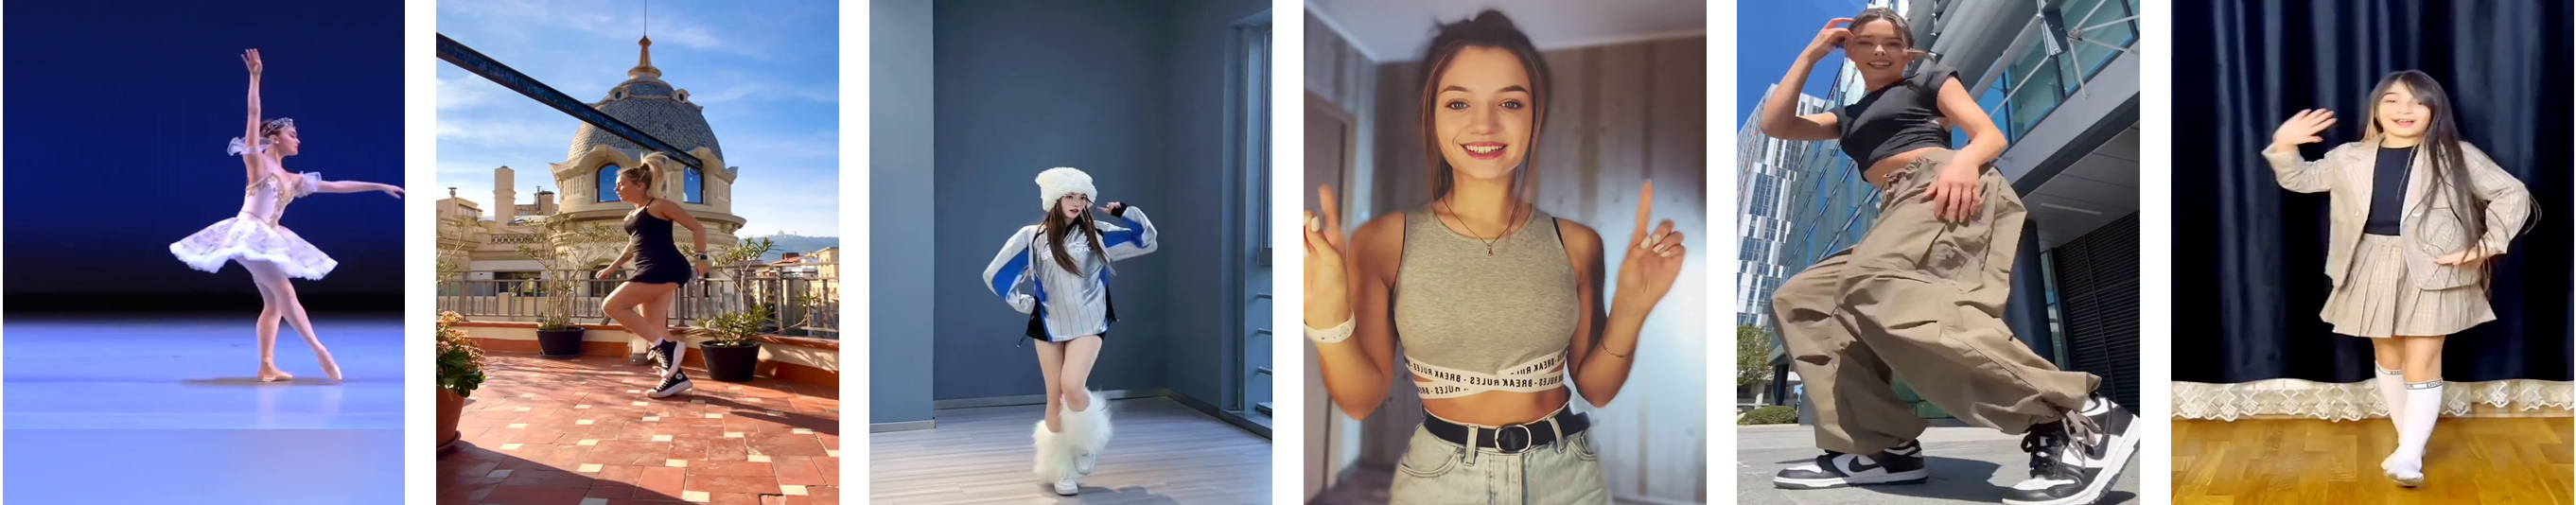
\includegraphics[width=1.0\linewidth]{fig/dataset.png}
%   \caption{Representative images of the proposed wild testing dataset.}
%   \label{fig:dataset}
%   \vspace{-5mm}
% \end{figure}

\section{Experiments}
\label{sec:exp}

\subsection{Implementations}
\textbf{Dataset.}
We have curated an in-the-wild dataset comprising approximately 5,000 high-fidelity authentic human videos sourced from reputable online repositories, encompassing a total of 1 million frames. 
The dataset is segmented as follows: Bilibili (2540 videos), Kuaishou (920 videos), Tiktok \& Youtube (1438 videos), and Xiaohongshu (430 videos). 
These videos feature individuals of varying ages, ethnicities, and genders, depicted in full-body, half-body, and close-up shots, set against diverse indoor and outdoor backdrops.
In order to enhance our model's capacity to analyze a wide range of human movements and attire, we have included footage of dancers showcasing various dance forms in diverse clothing styles. 
In contrast to existing datasets characterized by pristine backgrounds, our dataset capitalizes on the diversity and complexity of backgrounds to aid our model in effectively distinguishing the foreground human subjects from their surroundings.
To maintain fairness and align with established benchmarks in the field of image animation, the identical test set as utilized in MagicAnimate~\cite{xu2023magicanimate} has been employed for TikTok evaluation.

\begin{table}[!t]
\centering
\begin{tabular}{c|cccc|ccc}
\hline
Method          & L1 $\downarrow$ & PSNR $\uparrow$ & SSIM $\uparrow$ & LPIPS $\downarrow$  & FID-VID $\downarrow$ & FVD $\downarrow$ \\ \hline
MRAA  & 3.21E-04        & 29.39           & 0.672           & 0.296              & 54.47                           & 284.82           \\
DisCo             & 3.78E-04            & 29.03             & 0.668             & 0.292                            & 59.90                  & 292.80              \\
MagicAnimate  & 3.13E-04    & 29.16           & 0.714           & 0.239              & 21.75                          & 179.07           \\
Animate Anyone  & -            & 29.56             & 0.718             & 0.285                & -                                & 171.9              \\
Ours & 3.02E-04            & 29.84             & 0.773            & 0.235                             & 26.14                  & 170.20   \\
Ours*  & \textbf{2.94E-04}            & \textbf{29.91}             & \textbf{0.802}            & \textbf{0.234}                             & \textbf{21.07}                  & \textbf{160.82}         \\\hline
\end{tabular} 
\vspace{1mm}
\caption{Quantitative comparisons on Tiktok dataset.
* indicates that the proposed approach is fine-tuned on the Tiktok training dataset.}
\vspace{-4mm}
\label{tab:quantitative_tiktok}
\end{table}

\begin{figure*}[!t]
  \centering
  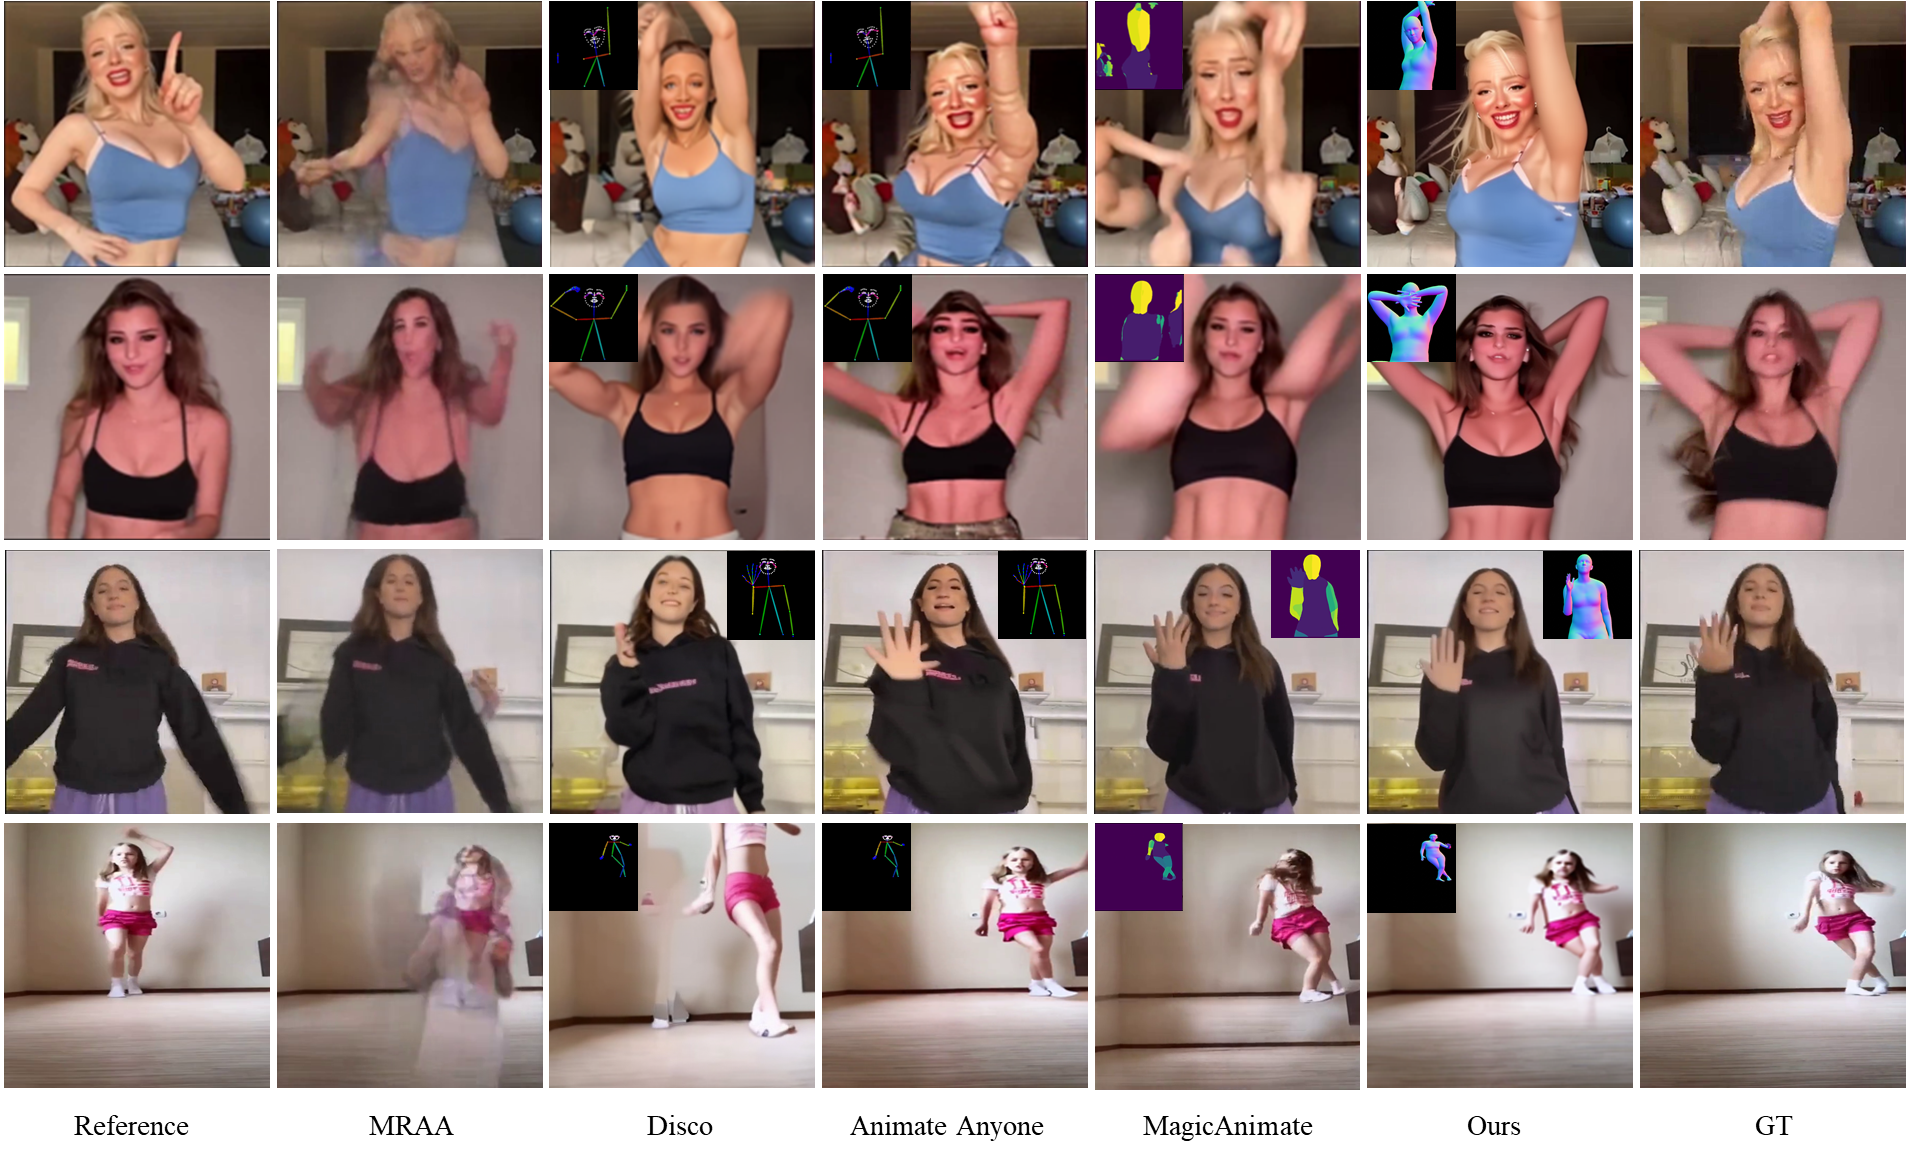
\includegraphics[width=\textwidth]{fig/qualitative_comparisons.png}
  \caption[]{Qualitative comparisons between our and the state-of-the-art approaches on TikTok and proposed unseen dataset.}
  \vspace{-4mm}
  \label{fig:qualitative_comparisons}
\end{figure*}

\textbf{Implementation.} 
Our experiments were facilitated by the computational power of 8 NVIDIA A100 GPUs. 
The training regimen is structured in two phases: initially, we processed individual video frames—sampling, resizing, and center-cropping them to a uniform resolution of 768x768 pixels. 
This stage spanned 60,000 steps with a batch size of 32. Subsequently, we dedicated attention to the temporal layer, training it over 20,000 steps with sequences of 24 frames and a reduced batch size of 8 to enhance temporal coherence. Both stages adhered to a learning rate of 1e-5.
During inference, to achieve continuity over extended sequences, we employed a temporal aggregation method, which facilitated the seamless integration of results from distinct batches, thereby generating longer video outputs. 

\begin{figure*}[!t]
  \centering
  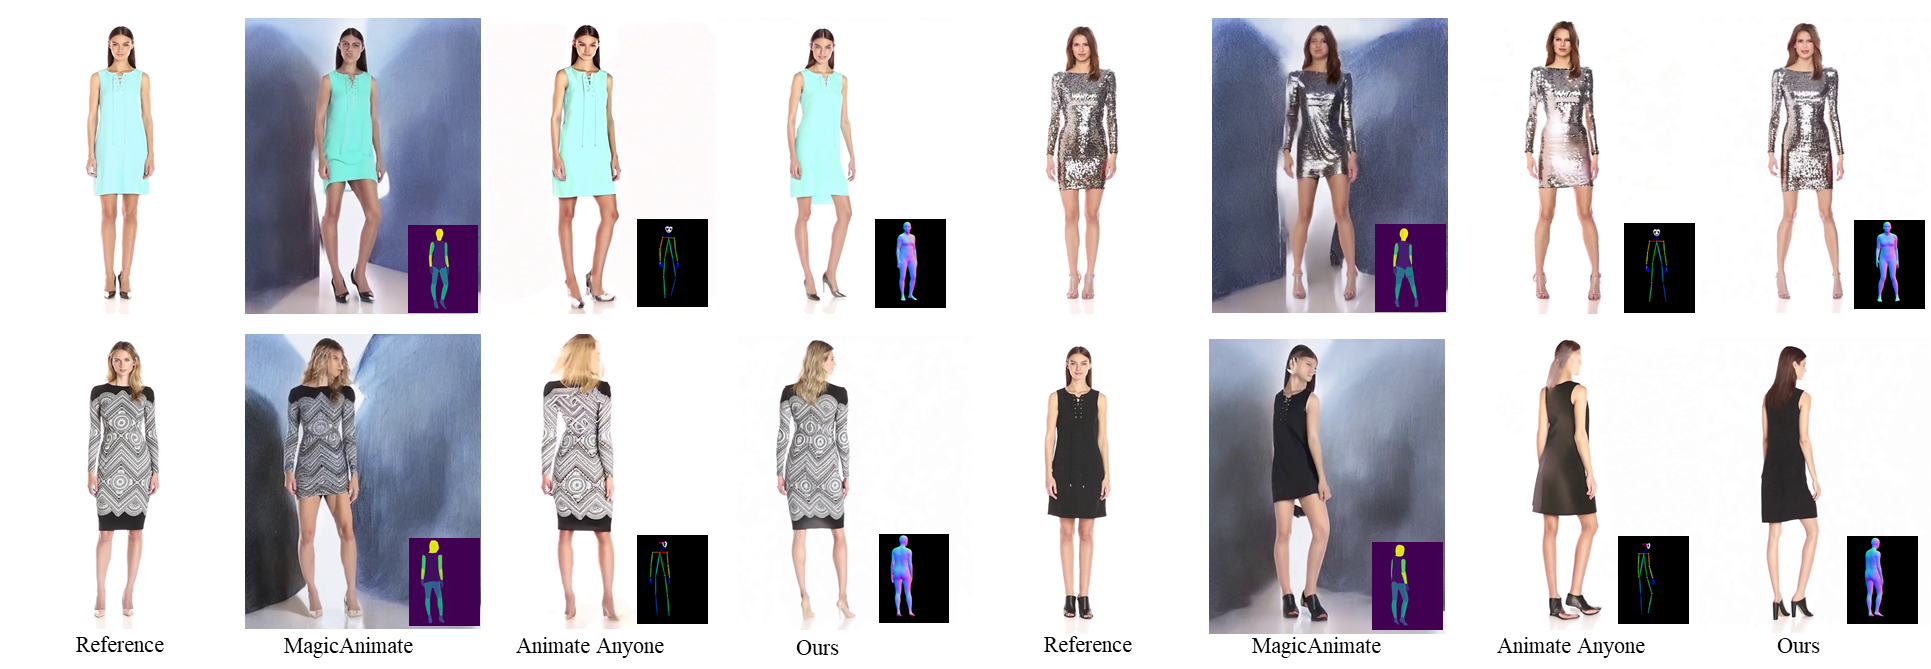
\includegraphics[width=\textwidth]{fig/fig_comp_ubc.png}
  \caption[]{Qualitative comparisons between our and the state-of-the-art approaches on UBC fashion video datasets.}
  \label{fig:ubc_data}
\end{figure*}

\begin{figure*}[!t]
  \centering
  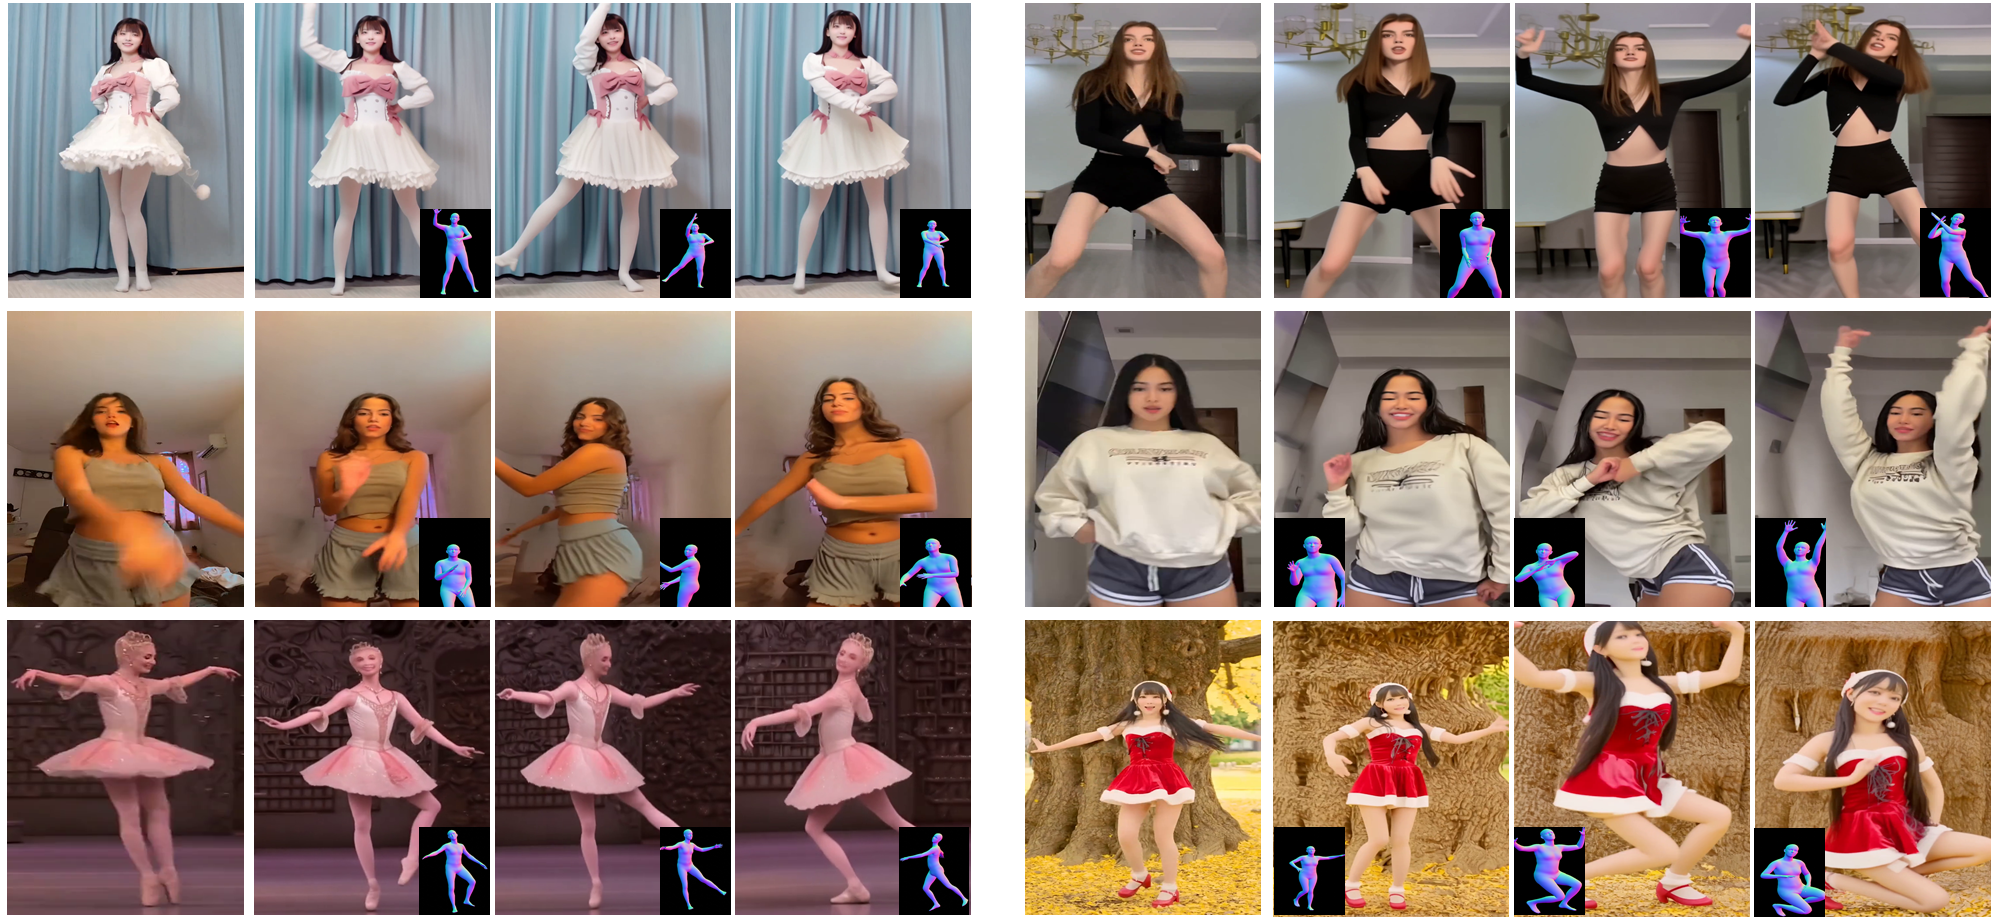
\includegraphics[width=\textwidth]{fig/fig_wild_results.png}
  \caption[]{More qualitative results of our approach on the proposed unseen dataset.}
  \vspace{-4mm}
  \label{fig:wild_data}
\end{figure*}

\subsection{Comparisons}
\textbf{Baselines.} We perform a comprehensive comparison with several state-of-the-art methods for human image animation: (1) MRAA~\cite{siarohin2021motion} is state-of-the-art GAN-based animation approaches, which estimate optical flow from driving sequences to warp the source image and then inpaint the occluded regions using GAN models. (2) DisCo~\cite{wang2023disco} is the state-of-the-art diffusion-based animation method that integrates disentangled condition modules for pose, human, and background into a pretrained diffusion model to implement human image animation. (3) MagicAnimate~\cite{xu2023magicanimate} and Animate Anyone~\cite{hu2023animate} are newer diffusion-based animation methods that employ more complex model structure and train on more general data which makes them perform quite well on TikTok dataset.
In all the qualitative (video and visual) comparative experiments, we employed the open-source implementation of Animate Anyone from MooreThreads\footnote{\tiny Animate Anyone: \url{https://github.com/MooreThreads/Moore-AnimateAnyone}} and MagicAnimate from the original authors\footnote{\tiny MagicAnimate: \url{https://github.com/magic-research/magic-animate}}. 
For all quantitative experimental comparisons, we directly referenced the relevant statistics from the original literature.

\begin{table}[!t]
\centering
\begin{tabular}{c|cccc}
    \hline
    Method          & PSNR $\uparrow$ & SSIM $\uparrow$ & LPIPS $\downarrow$ & FVD $\downarrow$ \\ \hline
    MRAA    & -          & 0.663           & 0.311           & 321.5                                   \\
    DisCo & 28.32          & 0.694           & 0.286          & 295.4    \\ 
    MagicAnimate & 29.14          & 0.713           & 0.235          & 193.6    \\ 
    Animate Anyone  & 28.86  &  0.727  & 0.242 & 199.2\\
    Ours  & \textbf{29.87}          & \textbf{0.806}           & \textbf{0.211}          & \textbf{173.5}\\ \hline
\end{tabular} 
\vspace{1mm}
\caption{Quantitative comparisons on proposed unseen dataset.}
\vspace{-4mm}
\label{tab:quantitative_wild}
\end{table}

\begin{table}[!t]
\centering
% \caption{Comparison of different methods on Image and Video metrics.}
\begin{tabular}{c|cccc|cc}
\hline
Method          & L1 $\downarrow$ & PSNR $\uparrow$ & SSIM $\uparrow$ & LPIPS $\downarrow$  & FID-VID $\downarrow$ & FVD $\downarrow$ \\ \hline
Ours (w/o. SMPL)  & 4.83E-04        & 28.57           & 0.672           & 0.296                  & 30.06                & 192.34          \\

Ours (w/o. geo.)  & 4.06E-04    & 28.78          & 0.714           & 0.276                        & 29.75                & 189.07           \\
Ours (w/o. skl.) & 3.76E-04            & 29.05            & 0.724             & 0.264            & 34.12                               & 184.24 \\
Ours & 3.02E-04          & 29.84           & 0.773            & 0.235          &  26.14                  & 170.20            \\\hline
\end{tabular}
\vspace{1mm}
\caption{Ablation study on different motion guidance.
``w/o. SMPL'' denotes a scenario where only the skeleton map is utilized as the motion condition.
``w/o. geo.'' indicates the model configuration that disregards geometric information, specifically depth and normal maps, as components of the motion condition.
``w/o. skl.'' describes the condition where the model solely relies on SMPL-derived inputs (including depth, normal, and semantic maps) for motion guidance.
``ours'' signifies the proposed approach that integrates both SMPL and skeleton derived motion condition.
}
\vspace{-4mm}
\label{tab:guidance_ablation}
\end{table}

\textbf{Evaluation metrics.} 
Our evaluation methodology adheres to the established metrics utilized in existing research literature.
Specifically, we assess both single-frame image quality and video fidelity. 
The evaluation of single-frame quality incorporates metrics such as the L1 error, Structural Similarity Index (SSIM)~\cite{wang2004image}, Learned Perceptual Image Patch Similarity (LPIPS)~\cite{zhang2018unreasonable}, and Peak Signal-to-Noise Ratio (PSNR)~\cite{5596999}. 
Video fidelity, on the other hand, is evaluated through the Frechet Inception Distance with Fréchet Video Distance (FID-FVD)~\cite{ijcai2019p276} and Fréchet Video Distance (FVD)~\cite{unterthiner2018towards}.

\textbf{Evaluation on benchmark dataset.}
Table~\ref{tab:quantitative_tiktok} presents a concise quantitative analysis of various methods evaluated on the TikTok dataset, focusing on key metrics such as L1 loss, PSNR, SSIM, LPIPS, FID-VID, and FVD. 
The proposed method, both in its original and fine-tuned (* indicated) forms, demonstrates superior performance across most metrics, particularly highlighting its effectiveness in achieving lower L1 loss, higher PSNR and SSIM values, and reduced LPIPS, FID-VID, and FVD scores. 
Notably, the fine-tuned version of our approach shows the best overall results, indicating the benefits of dataset-specific optimization. 
Figure~\ref{fig:qualitative_comparisons} and Figure~\ref{fig:ubc_data} provides additional qualitative comparison on such benchmark.

\textbf{Evaluation on Proposed Unseen Dataset.}
In order to further compare the robustness of various methods, distinct from datasets such as TikTok and UBC fashion that exhibit domain proximity, we have constructed a testing dataset comprising 100 high-fidelity authentic human videos sourced from online repositories.
These videos exhibit significant variations in the shape, pose, and appearance of the individuals depicted.
Figure~\ref{fig:wild_data} and Figure~\ref{fig:unseen_data} provides some qualitative comparison of the unseen dataset along with the statistical comparison presented in Table~\ref{tab:quantitative_wild}, collectively illustrate the efficacy of the proposed approach in generalizing to unseen domains.


\begin{table}[!t]
\centering
\begin{tabular}{c|cccc|cccc}
\hline
Method          & L1 $\downarrow$ & PSNR $\uparrow$ & SSIM $\uparrow$ & LPIPS $\downarrow$ &  FID-VID $\downarrow$ & FVD $\downarrow$ \\ \hline
w/o.  & 3.21E-04        & 29.44           & 0.752           & 0.248                      & 25.36                & 174.46           \\
w/.  & 3.02E-04           & 29.84             & 0.785            & 0.235                              & 21.28                  & 170.20             \\\hline
\end{tabular} 
\vspace{1mm}
\caption{Ablation study on guidance self-attention.}
\vspace{-4mm}
\label{tab:guidance_attention}
\end{table}

\begin{figure}[!t]
  \centering
  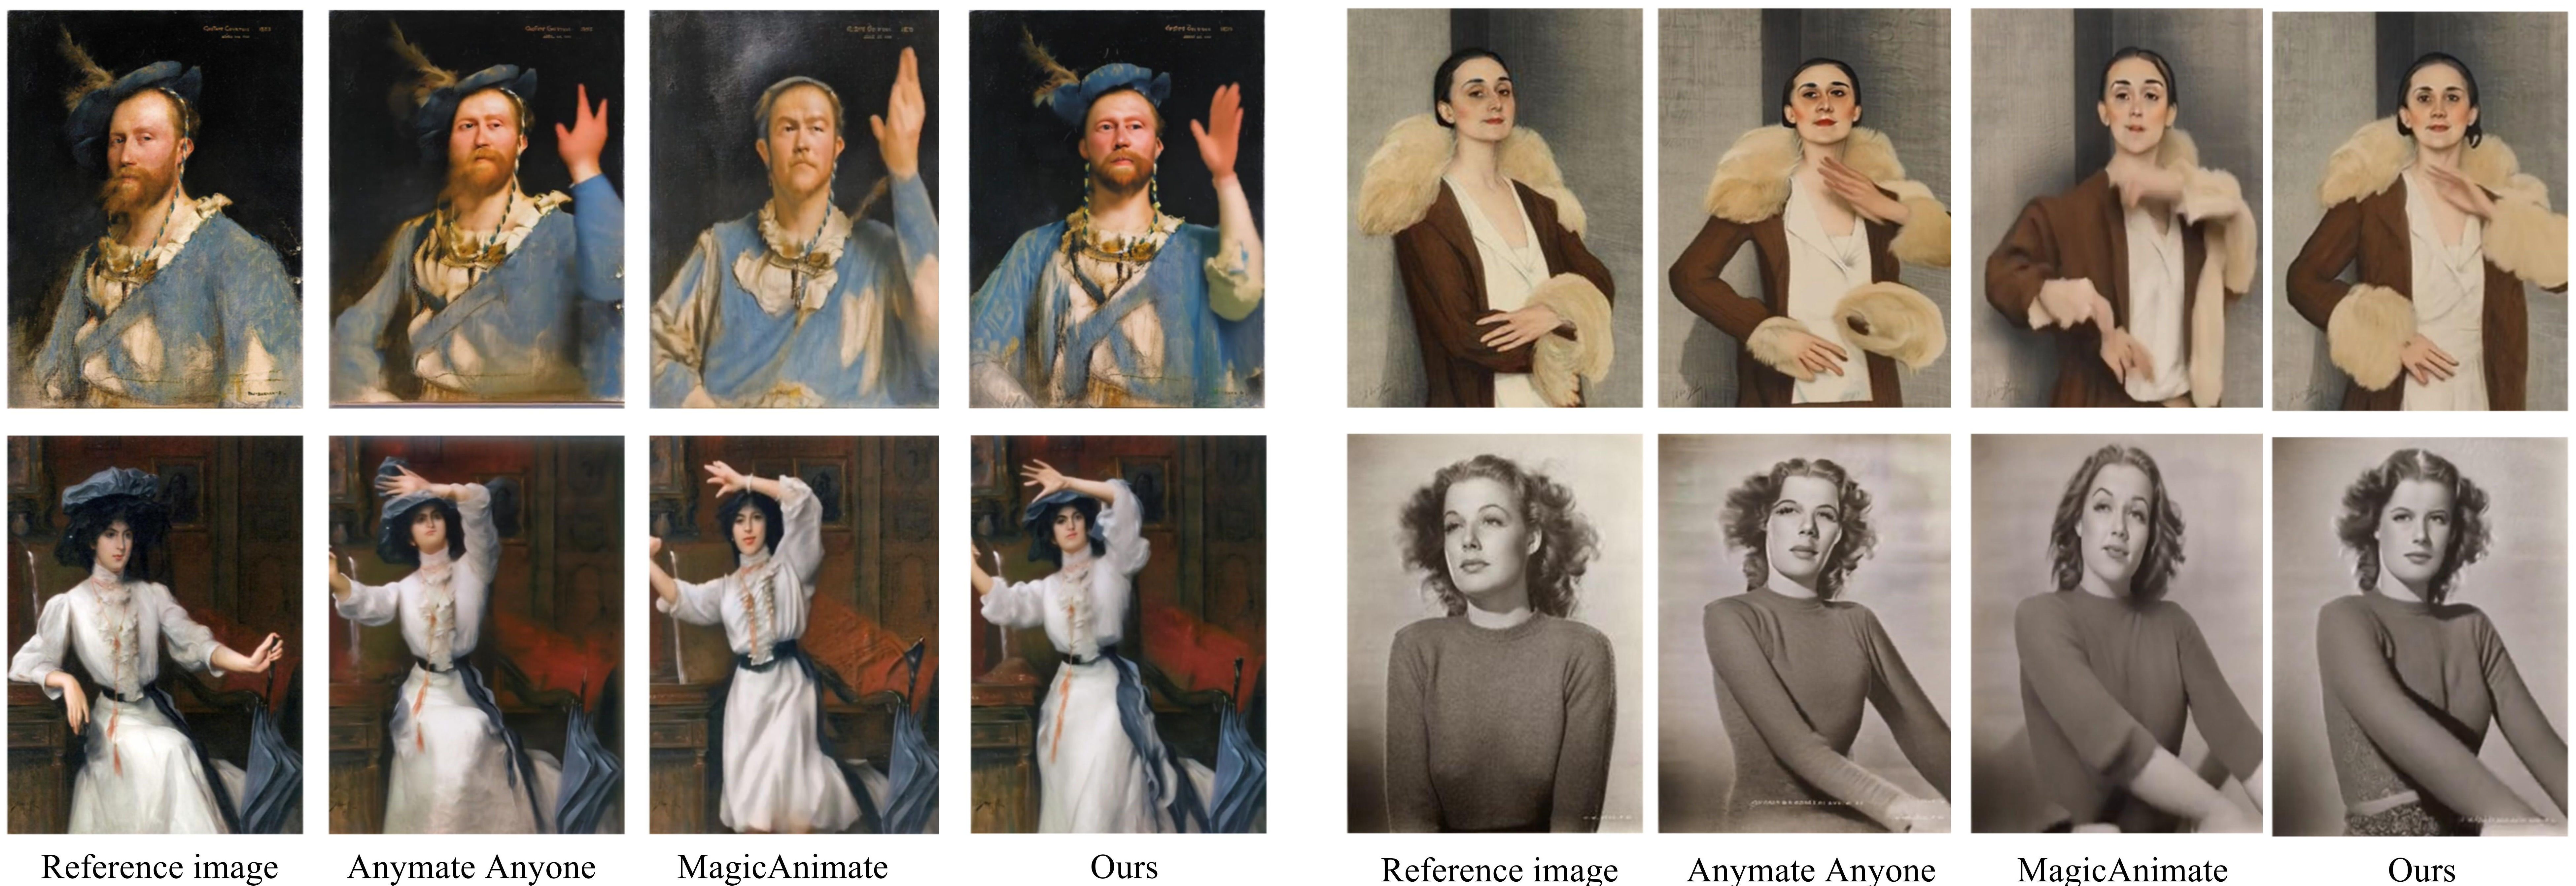
\includegraphics[width=1.0\linewidth]{fig/unseen.jpg}
  \caption{The qualitative comparison of animating unseen domain images.}
  \label{fig:unseen_data}
\end{figure}

\begin{figure}[!t]
  \centering
  \includegraphics[width=1.0\linewidth]{fig/cross_id.jpg}
  \caption{The demonstration of cross ID animation from the proposed approach.}
  \vspace{-4mm}
  \label{fig:cross_id}
\end{figure}

\begin{figure}[!t]
  \centering
  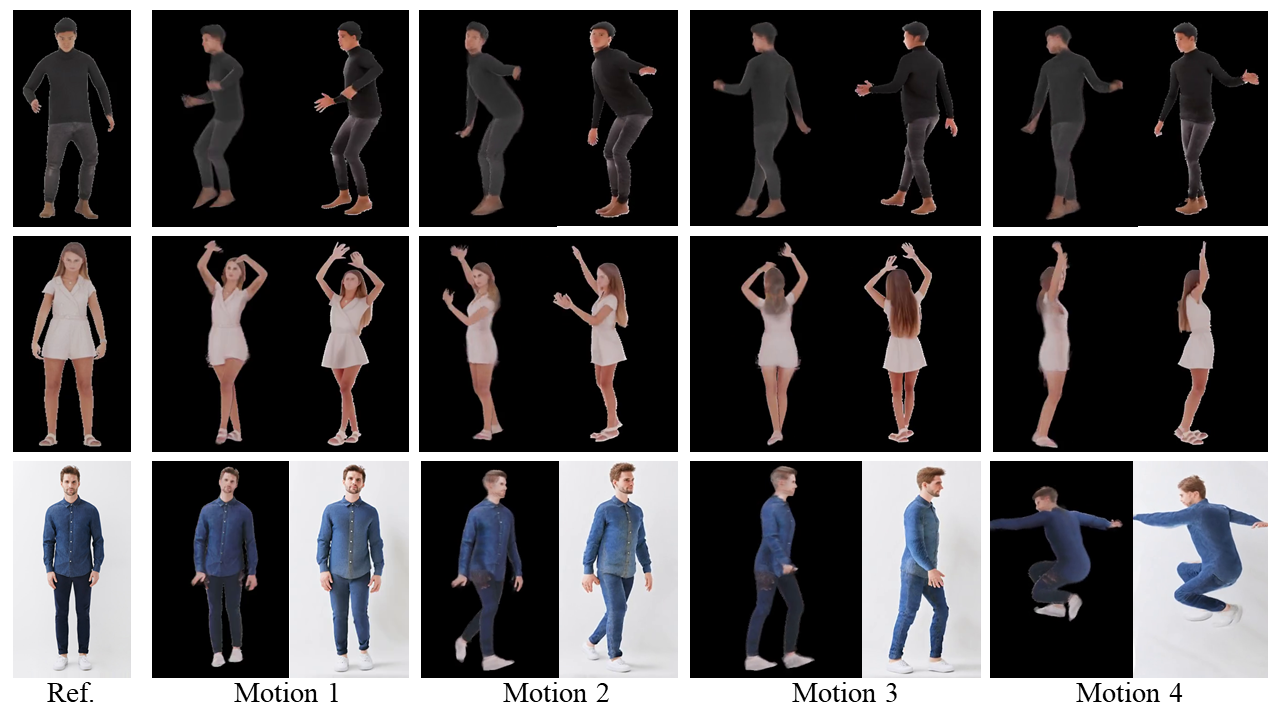
\includegraphics[width=1.0\linewidth]{fig/comp_sherf.png}
  \caption{Comparision between SHERF (left) and ours (right).}
  \vspace{-4mm}
  \label{fig:comp_sherf}
\end{figure}

\begin{figure}[!t]
  \centering
  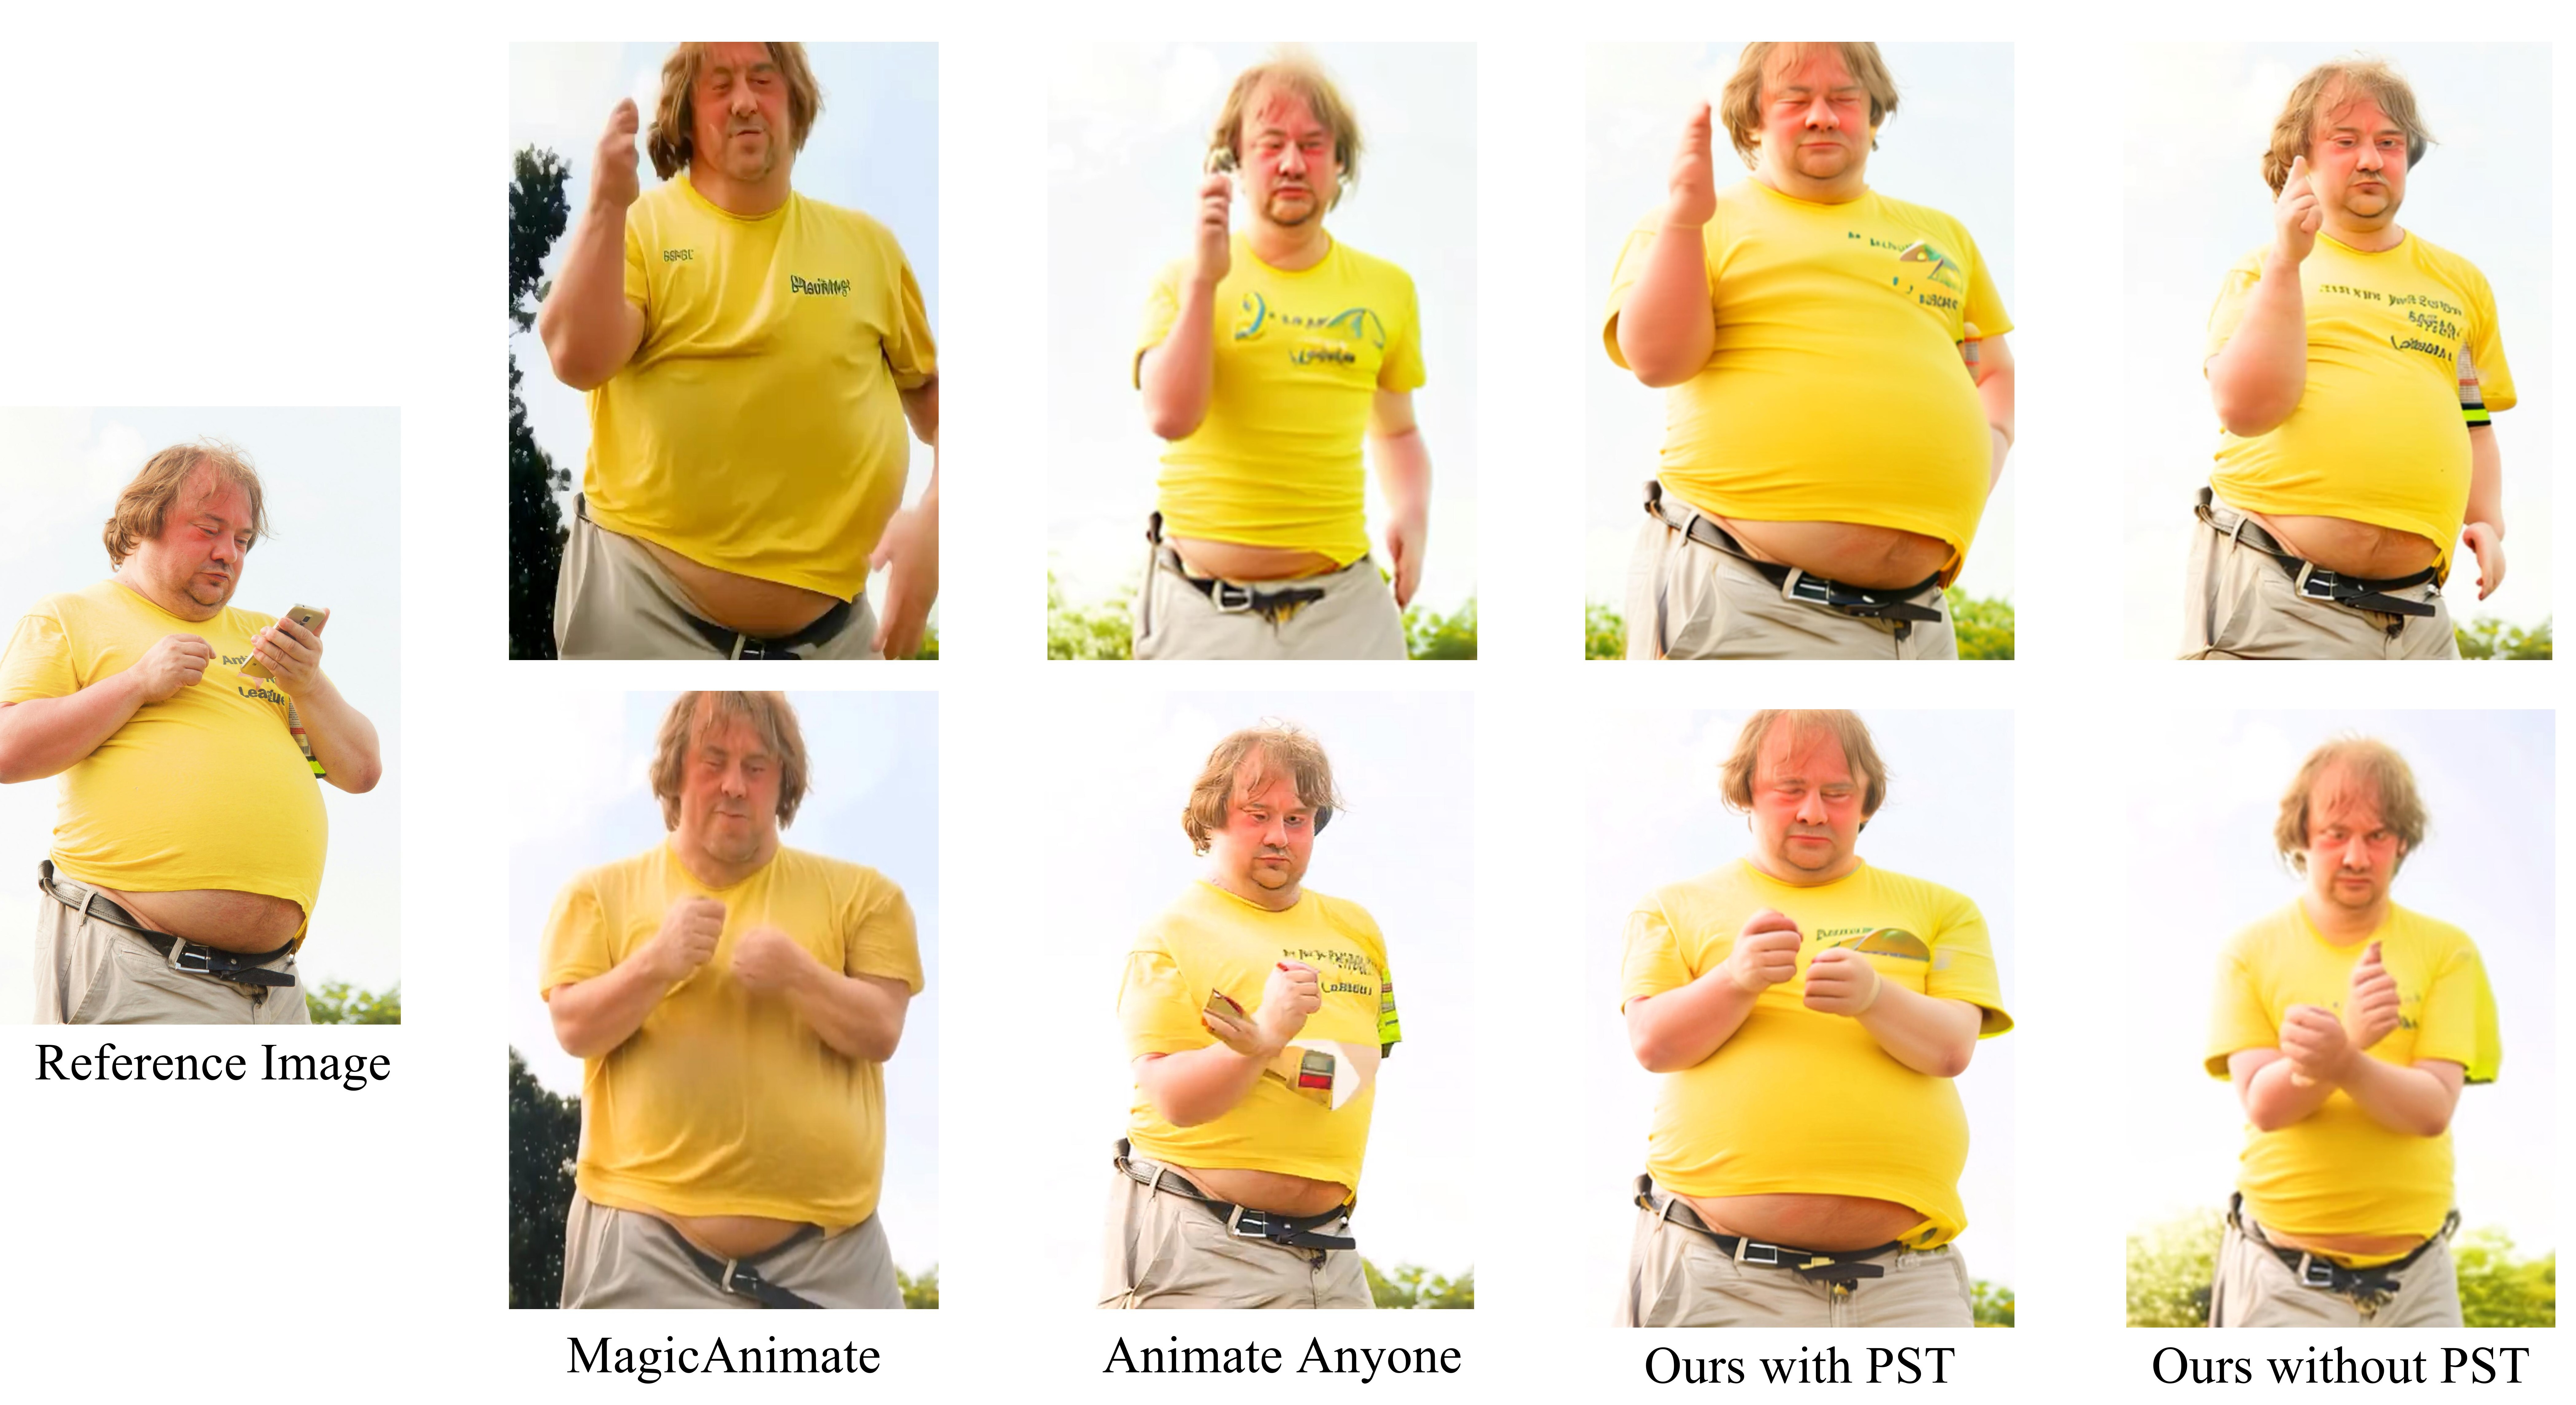
\includegraphics[width=0.8\linewidth]{fig/shape_variance.jpg}
  \caption{The comparison on the shape variance data.}
  \label{fig:shape_variance}
\vspace{-4mm}  
\end{figure}



\textbf{Cross ID Animation.}
As shown in Figure~\ref{fig:cross_id}, a comparative analysis is conducted between our approach and state-of-the-art baseline methods for cross-identity animation, specifically focusing on the task of animating reference images through motion sequences derived from disparate videos.

\textbf{Multi-view Animation.}
Although our method may not match the direct rendering of 3D human representations for consistent novel views, we employ a sequence of SMPLs for multi-view consistent motion guidance and utilize generative models to achieve satisfactory multi-view results.  As shown in Figure~\ref{fig:comp_sherf}, we compare the results of our multi-view animation with a representative single-image to 3D human reconstruction method, SHERF~\cite{hu2023sherf}.

\subsection{Ablation Studies}
\textbf{Different Conditions from SMPL.}
As shown in Table~\ref{tab:guidance_ablation}, the statistics demonstrate that the full configuration of the proposed method (``ours'') obviously outperforms other variants in terms of image quality and fidelity, and video consistency and realism. 
The ablation components, ``w/o SMPL'', ``w/o geometry'', and ``w/o skeleton'', show progressively improved performance as more components are included.
Specifically, SMPL obviously brings more gains in PSNR (1.27 v.s. 0.48) and SSIM (0.10 v.s. 0.05) gains than a skeleton, which means better preserving the shape alignment and motion guidance.
Moreover, it is noteworthy that the incorporation of both the SMPL and skeleton models leads to additional improvements. 
Specifically, the skeleton model exhibits advantages in providing refined motion guidance for facial and hand regions.
Meanwhile, Figure~\ref{fig:ablation_motion} qualitative demonstrates the effectiveness of different conditions from SMPL.

\textbf{Guidance Self-Attention.}
Table~\ref{tab:guidance_attention} presents the findings of an ablation study conducted on guidance self-attention. 
The results indicate that the inclusion of guidance attention leads to superior performance compared to the absence of such attention, as evidenced by improvements across all evaluated metrics. 
As shown in Figure~\ref{fig:ablation_guidance}, we provide additional qualitative results of the guidance self-attention.

\begin{figure}[!t]
  \begin{minipage}{0.48\textwidth}
     \centering
    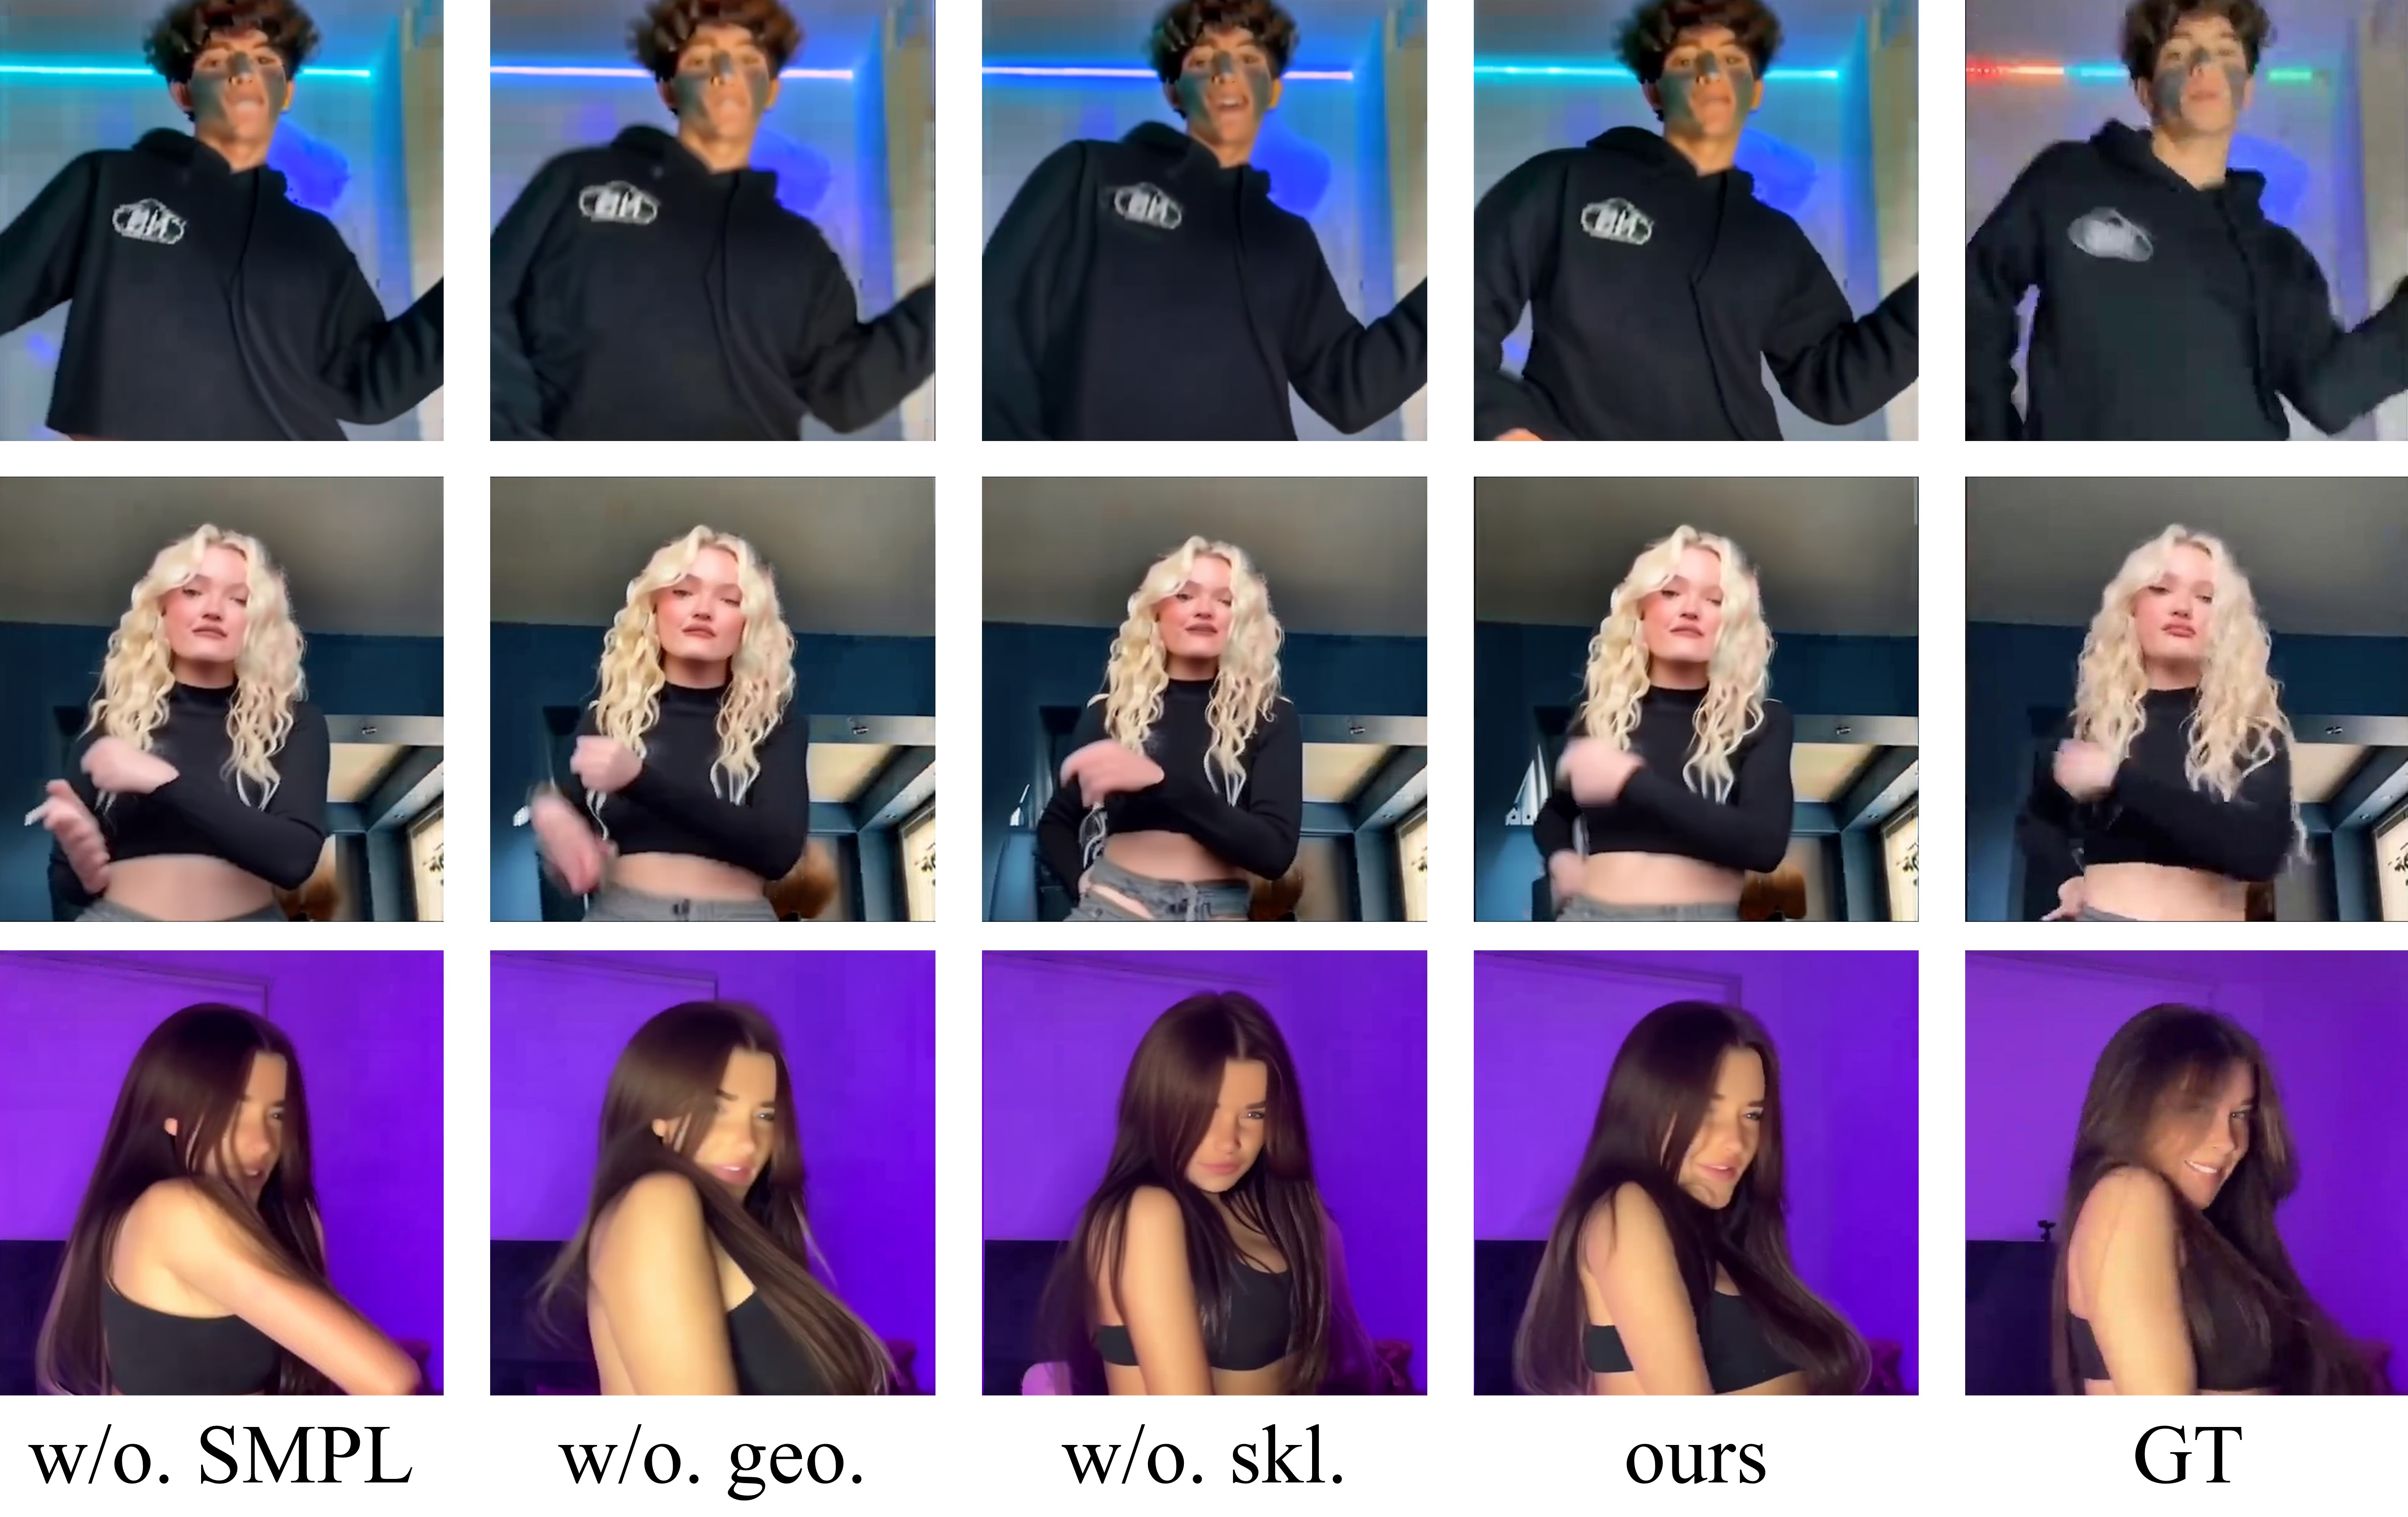
\includegraphics[width=1.0\textwidth]{fig/guidance_ablation.jpg}
    \caption{Ablation analysis on different motion conditions. geo. refers to the geometry. skl. is the skeleton condition.}
    \label{fig:ablation_motion}
    
  \end{minipage}
  \hfill
   \begin{minipage}{0.48\textwidth}
    \centering
    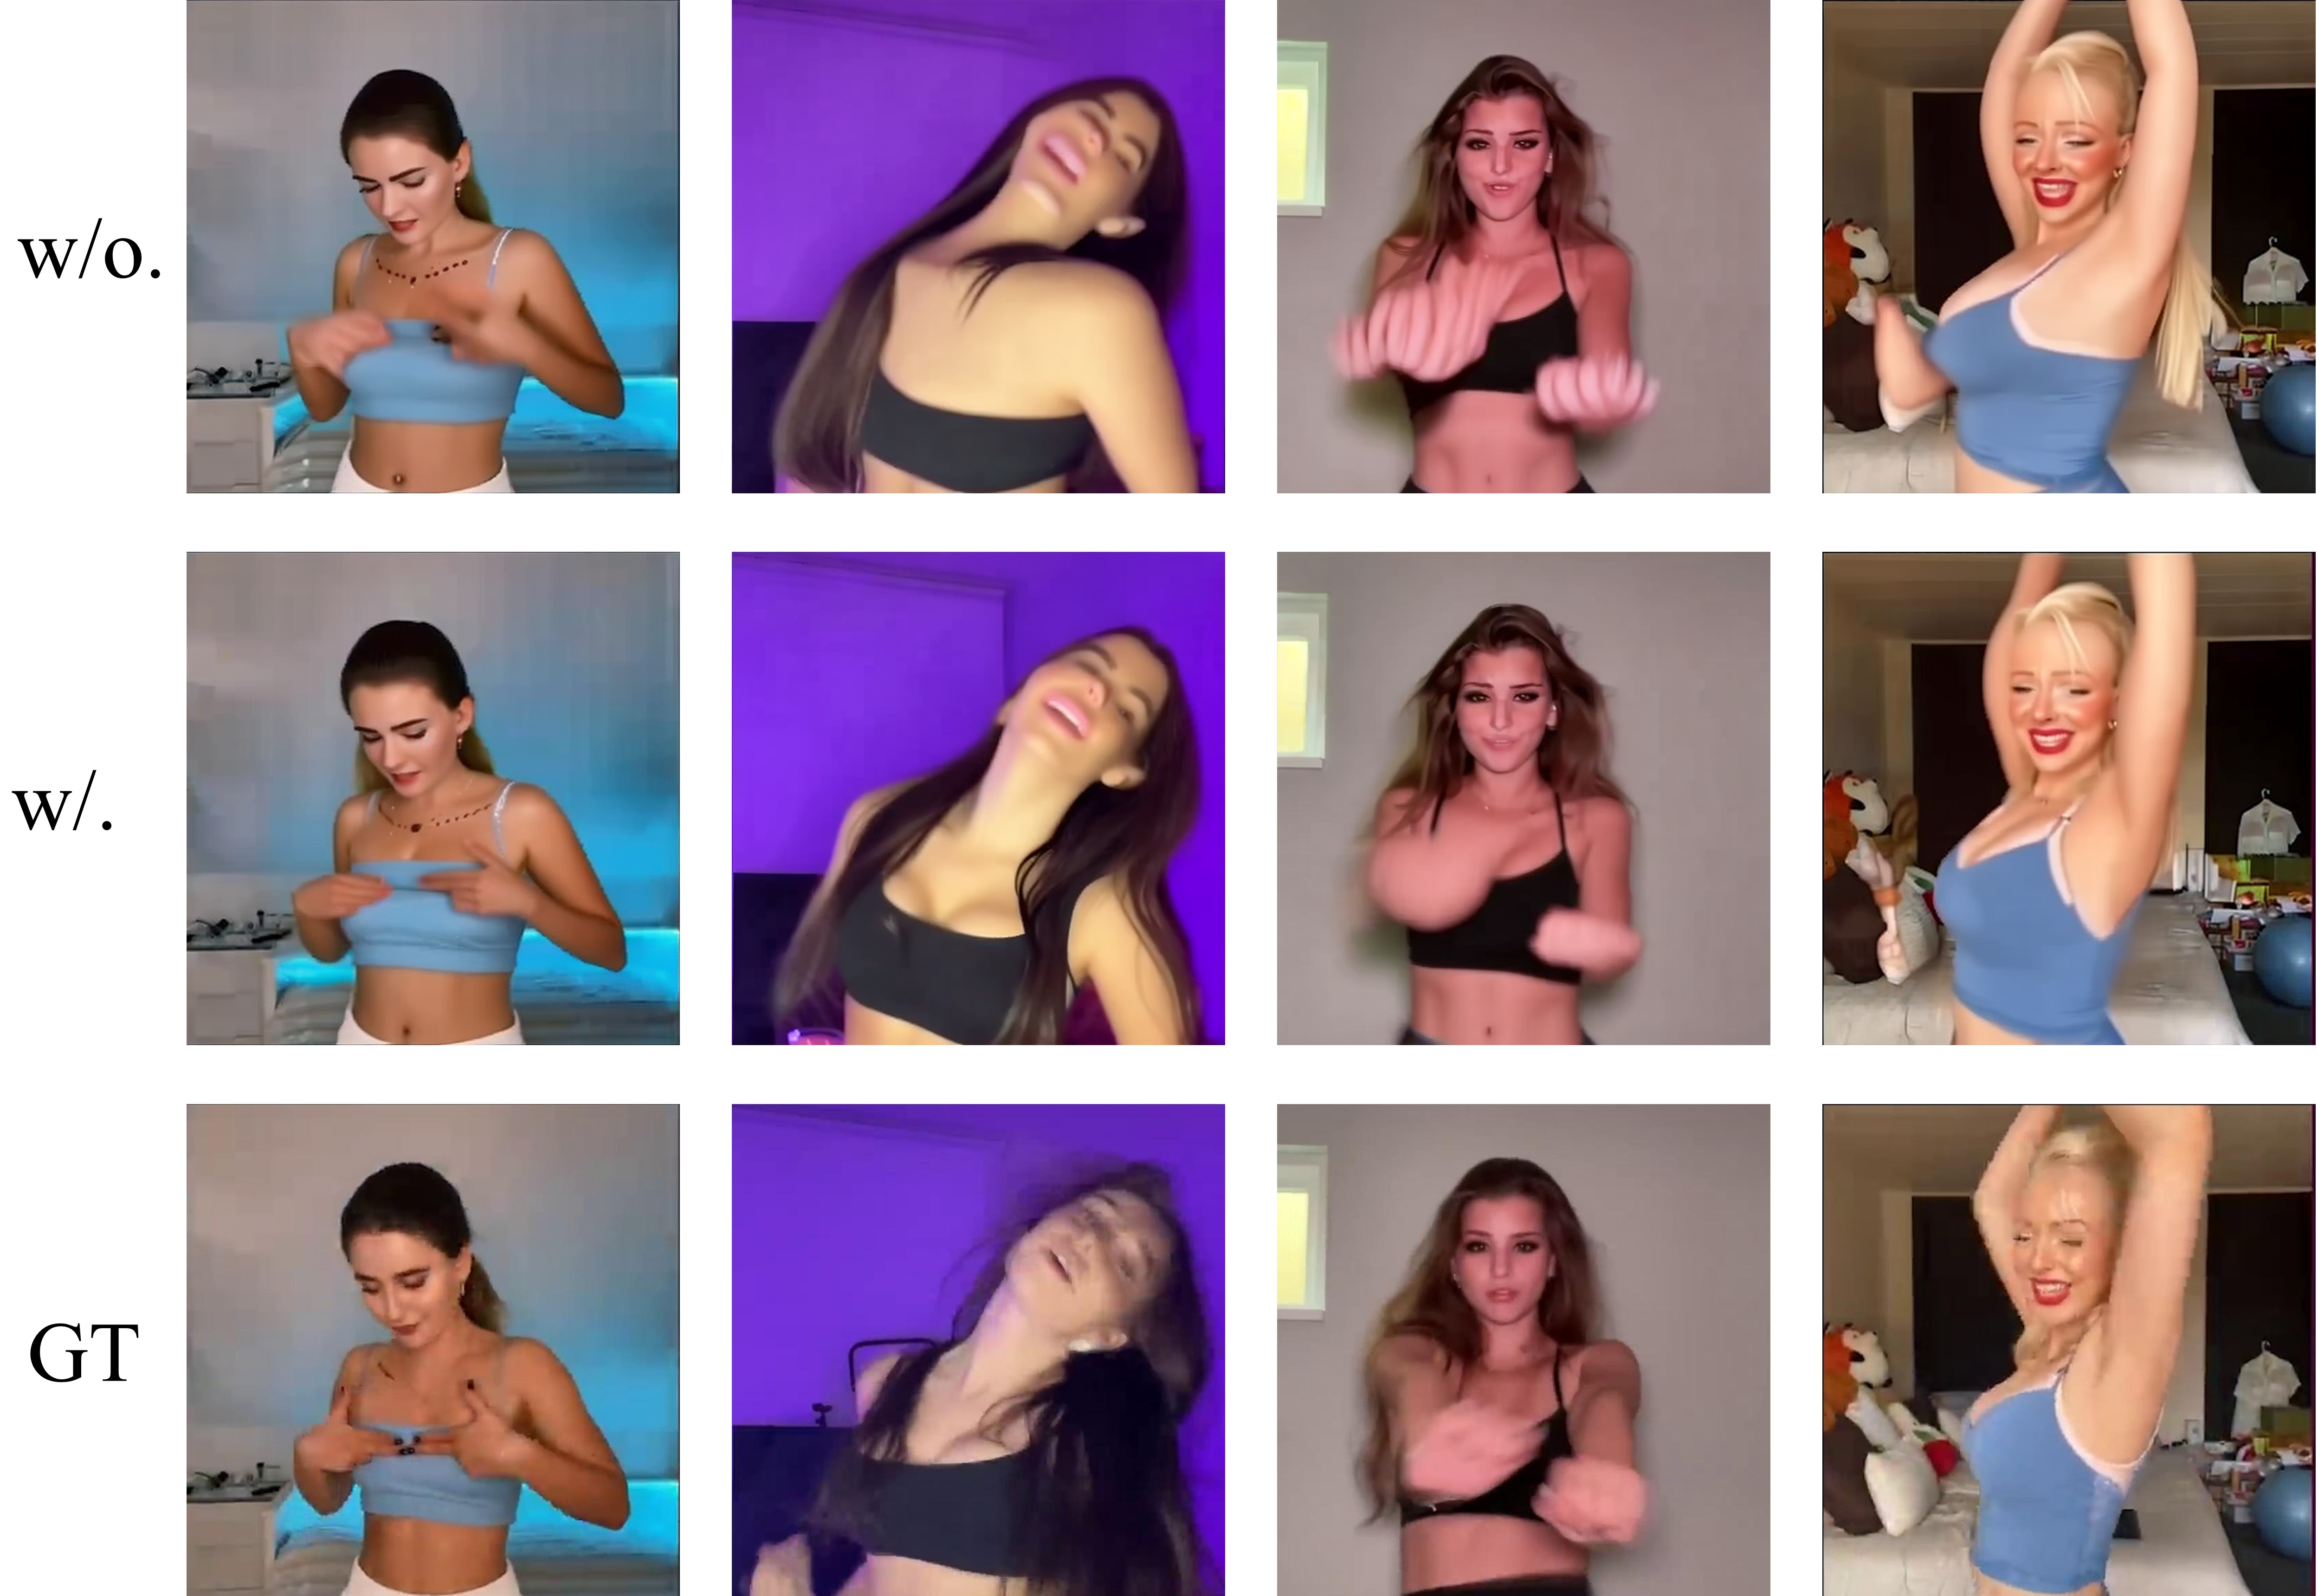
\includegraphics[width=0.9\textwidth]{fig/attention_ablation.jpg}
    \caption{Effect of guidance attention. w/. and w/o. indicate the guidance with and without self-attention.}
    \label{fig:ablation_guidance}
  \end{minipage}
\end{figure}

\textbf{Parametric Shape Alignment.}
As shown in Figure~\ref{fig:shape_variance},  we take an ablation study on shape parameter alignment between reference humans' SMPL model and driving videos' SMPL sequence. To highlight the effect, we use an individual with an extreme figure as the reference image and a common human dancing video as input. In comparison to other methods, our results from parametric shape alignment in the third row exhibit the most consistent shape and figure alignment with the reference image.

\textbf{Efficiency Analysis.}
Table~\ref{tab:efficiency} presents an efficiency analysis of our proposed approach, detailing the GPU memory requirements and time consumption for different steps, including parametric shape transfer, rendering per frame, and inference per frame.

\begin{table}[!t]
\centering
\begin{tabular}{c|ccccc}
\hline
Method          & GPU memory (GB) & & & & Time (sec) \\ \hline
Parametric shape transfer    &   3.24     & & & & 0.06 \\
Rendering (per frame) &  2.86    & & & & 0.07 \\
Inference (per frame)  & 19.83       & & & & 0.52 \\\hline
\end{tabular} 
\vspace{1mm}
\caption{Efficiency analysis of different steps of the proposed approach.} 
\label{tab:efficiency}
\vspace{-4mm}  
\end{table}

\subsection{Limitations and Future Works}
Despite the enhanced shape alignment capabilities and motion guidance offered by the human parametric SMPL model, its modeling capacity for faces and hands is limited. 
Consequently, the guidance effect for faces and hands does not match the efficacy of feature-based methods. This limitation underpins the incorporation of DWpose as an additional constraint for facial and hand modeling. 
As illustrated in Figure~\ref{fig:motion_guidance}, the self-attention mechanism further amplifies the saliency of faces and hands within the skeleton map. 
However, it is important to note that since SMPL and DWpose are solved independently, a potential discrepancy in consistency between them exists. 
Although this discrepancy did not manifest significantly in our experiments, it nonetheless introduces a potential source of error.